\documentclass[aspectratio=169,11pt,t]{beamer}
% ============================================================
%  ksa-cs-v2: ksa-cs-lecture-template.tex 스타일 + 한글, v2 덱(16:9)용.
%    - 짙은 네이비 헤드라인 (섹션 이름 + 프레임마다 점)
%    - 꽉 찬 파란 제목 막대, 둥근 그림자 블록
%    - 한글: Noto Sans CJK KR (fontspec)
%  사용:
%    \documentclass[aspectratio=169,11pt,t]{beamer}
%    \input{<..>/theme/ksa-cs-v2.tex}
%  ksa-theme.tex 의 매크로(\kb \kq, ksablue/ksared 등)도 같은 이름으로 둔다
%  -> v2 덱 본문을 거의 그대로 옮길 수 있다.
% ============================================================

\usepackage{fontspec}
\usepackage{amsmath,amssymb}
\usepackage{tikz}
\usepackage{listings}
\usepackage{graphicx}
\usepackage{booktabs}
\usepackage{varwidth}
% enumitem 은 넣지 않는다 (beamer 글머리표가 사라진다)

\defaultfontfeatures{Ligatures=TeX}
\setmainfont{Noto Sans CJK KR}
\setsansfont{Noto Sans CJK KR}
\setmonofont{Noto Sans Mono CJK KR}[Scale=0.92]
\usefonttheme{professionalfonts}

% ---------- 기본 틀 ----------
\usetheme{default}
\useinnertheme[shadow=true]{rounded}
\setbeamertemplate{navigation symbols}{}
\setbeamersize{text margin left=1em,text margin right=1em}

% ---------- 색 (템플릿 원본 값) ----------
\definecolor{navydark}{HTML}{191959}
\definecolor{navydim}{HTML}{8888B0}
\definecolor{navytitle}{HTML}{262686}
\definecolor{navyblue}{HTML}{3333B2}
\definecolor{blockbodybg}{HTML}{E9E9F3}
\definecolor{examplegreen}{HTML}{006000}
\definecolor{examplebg}{HTML}{E5EFE5}
\definecolor{alertred}{HTML}{BF0000}
\definecolor{alertbg}{HTML}{F9E5E5}
% ksa-theme.tex 와 같은 이름 (본문 호환)
\colorlet{ksablue}{navytitle}
\colorlet{ksabluedk}{navydark}
\definecolor{ksagold}{HTML}{D6CBB1}
\definecolor{ksagolddk}{HTML}{A9976B}
\colorlet{ksared}{alertred}
\definecolor{ksagray}{HTML}{5B5B5B}

\setbeamercolor{structure}{fg=navyblue}
\setbeamercolor{alerted text}{fg=alertred}
\setbeamercolor{frametitle}{bg=navytitle,fg=white}
\setbeamercolor{title}{fg=white,bg=navytitle}
\setbeamercolor{block title}{bg=navytitle,fg=white}
\setbeamercolor{block body}{bg=blockbodybg,fg=black}
\setbeamercolor{block title example}{bg=examplegreen,fg=white}
\setbeamercolor{block body example}{bg=examplebg,fg=black}
\setbeamercolor{block title alerted}{bg=alertred,fg=white}
\setbeamercolor{block body alerted}{bg=alertbg,fg=black}
\setbeamercolor{item}{fg=navyblue}
\setbeamertemplate{itemize item}[circle]
\setbeamertemplate{itemize subitem}[triangle]

% ---------- 헤드라인: miniframes (섹션 이름 + 점) ----------
\useoutertheme[subsection=false]{miniframes}
\setbeamerfont{section in head/foot}{size=\tiny}
\setbeamercolor{section in head/foot}{bg=navydark,fg=white}
\setbeamercolor{mini frame}{fg=white}
\setbeamertemplate{mini frames}[circle]

% ---------- 제목 막대: 폭 꽉 채움, 두 줄까지 ----------
\setbeamerfont{frametitle}{size=\normalsize,series=\bfseries}
\setbeamertemplate{frametitle}{%
  \nointerlineskip
  \begin{beamercolorbox}[wd=\paperwidth,ht=2.7ex,dp=1.1ex,leftskip=.3cm,rightskip=.3cm]{frametitle}%
    \usebeamerfont{frametitle}\insertframetitle
  \end{beamercolorbox}}

% ---------- 쪽 번호: 오른쪽 아래 ----------
\setbeamertemplate{footline}{%
  \hfill
  {\color{navydim}\scriptsize\insertframenumber\,/\,\inserttotalframenumber}%
  \hspace{3mm}\vspace{2mm}%
}

% ---------- 표지: 템플릿처럼 헤드라인은 그대로, 가운데 둥근 그림자 상자에 제목 한 줄 ----------
% 덱에서:  {\setbeamertemplate{footline}{}\begin{frame}[c,noframenumbering]\titlepage\end{frame}}
\setbeamercolor{title}{fg=white,bg=navyblue}
\makeatletter
\setbeamertemplate{title page}{%
  \vfill
  \centering
  \begin{minipage}{0.84\paperwidth}
  \begin{beamercolorbox}[wd=\linewidth,sep=7pt,center,rounded=true,shadow=true]{title}
    {\usebeamerfont{title}\inserttitle\par}%
    \ifx\insertsubtitle\@empty\else\vskip0.4em{\usebeamerfont{subtitle}\insertsubtitle\par}\fi
  \end{beamercolorbox}
  \end{minipage}\par\vskip1.6em
  {\usebeamerfont{author}\color{navytitle}\insertauthor\par}\vskip0.3em
  {\usebeamerfont{institute}\color{ksagray}\insertinstitute\par}
  \vfill
}
\makeatother
\setbeamerfont{title}{series=\bfseries,size=\Large}
\setbeamerfont{subtitle}{size=\normalsize}
\setbeamerfont{author}{size=\normalsize}
\setbeamerfont{institute}{size=\small}

% ksa-theme 호환: 덱이 \renewcommand{\ksacredit}{..} 를 해도 되게 (꼬리말에는 안 쓴다)
\newcommand{\ksacredit}{}

% ---------- 강조 ----------
\newcommand{\hl}[1]{\textcolor{alertred}{#1}}
\newcommand{\hlb}[1]{\textcolor{navyblue}{#1}}
\newcommand{\kb}[1]{\textbf{\color{ksablue}#1}}
\newcommand{\kq}[1]{\textbf{\color{ksared}#1}}

% ---------- 파이썬 코드 (템플릿과 같은 색) ----------
\definecolor{codekw}{HTML}{0033B3}
\definecolor{codebuiltin}{HTML}{BF0000}
\definecolor{codestr}{HTML}{067D17}
\definecolor{codecomment}{HTML}{8C8C8C}
\definecolor{codenum}{HTML}{1750EB}
\lstdefinestyle{py}{
  language=Python, basicstyle=\ttfamily\scriptsize,
  keywordstyle=\color{codekw}\bfseries, stringstyle=\color{codestr},
  commentstyle=\color{codecomment}\itshape, numberstyle=\color{codenum},
  emph={print,len,range,sum,input,int,str,float,list,dict,append,remove,sorted,abs,min,max},
  emphstyle=\color{codebuiltin}, showstringspaces=false, keepspaces=true,
  columns=fixed, basewidth=0.52em, aboveskip=1mm, belowskip=1mm, xleftmargin=2mm,
  breaklines=true
}
\lstset{style=py}

% 원본 덱 (ksa-theme): slides/v2/ml1/week14/tsne/ -- 그림은 거기 figs/ 를 그대로 쓴다
\setbeamerfont{author}{size=\normalsize}
\setbeamerfont{institute}{size=\small}
\graphicspath{{../../../v2/ml1/week14/tsne/figs/}{../../../assets/}}
\makeatletter
\newcommand{\markpage}[1]{\protected@write\@auxout{}{\string\newlabel{#1}{{\the\c@framenumber}{}}}\hypertarget{#1}{}}
\newcommand{\pref}[1]{\hyperlink{#1}{\textcolor{ksagolddk}{(p.\ref{#1})}}}
\makeatother

\renewcommand{\ksacredit}{Machine Learning and Deep Learning \,\textperiodcentered\, t-SNE}
\title{t-SNE 데이터 지도}
\subtitle{가까운 이웃은 지도에서도 이웃으로}
\author{Machine Learning and Deep Learning}
\institute{한국과학영재학교 (KSA)}
\date{}
\begin{document}
{\setbeamertemplate{footline}{}\begin{frame}[c,noframenumbering]\titlepage\end{frame}}


\section{질문}
% --- 오늘의 질문
\begin{frame}{오늘의 질문: 64차원 점 1,797개를 지도 한 장에?}
\vfill
\begin{columns}[c]
\column{0.32\linewidth}\centering
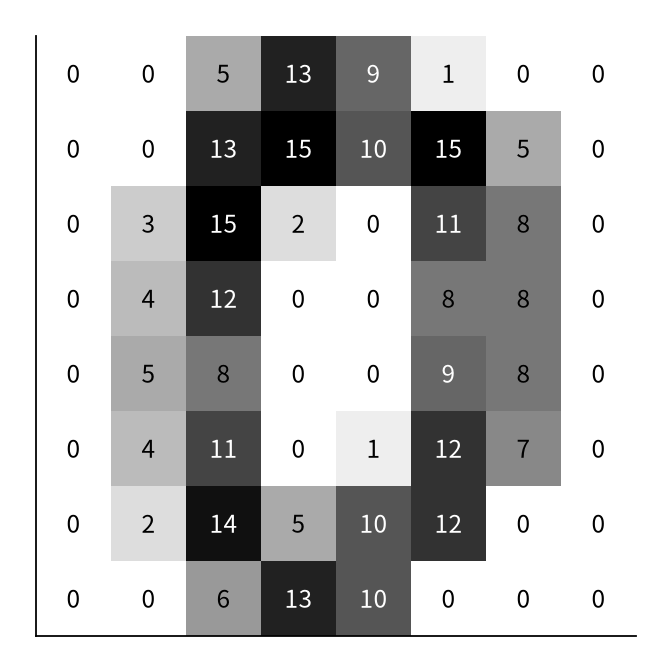
\includegraphics[width=\linewidth]{ts_digit.png}
\column{0.64\linewidth}
{\large 숫자 한 장 = 8 × 8 = 숫자 \kb{64}개}\\[0.2em]{\large = 64차원 공간의 점 하나}\\[0.6em]
{\large 1,797장을 2차원 지도에 그려}\\[0.2em]{\large \textbf{비슷한 것끼리 모였는지} 보고 싶다}\\[0.6em]
{\large PCA 두 축: 퍼짐의 28.5\% 만 남는다}
\end{columns}
\vfill
\note{손글씨 숫자 한 장은 8 곱하기 8, 숫자 64개입니다. 64차원 공간의 점 하나죠. 이런 점 1797개를 2차원 지도 한 장에 그려서, 비슷한 숫자끼리 모여 있는지 보고 싶습니다. 6주차 PCA로 두 축만 남기면 퍼짐의 28.5퍼센트만 남는다고 했습니다. 지도가 어떻게 보일까요?}
\end{frame}

\section{아이디어}
% --- PCA vs t-SNE
\begin{frame}{PCA 지도 vs t-SNE 지도}
\markpage{maps}
\vfill
\centering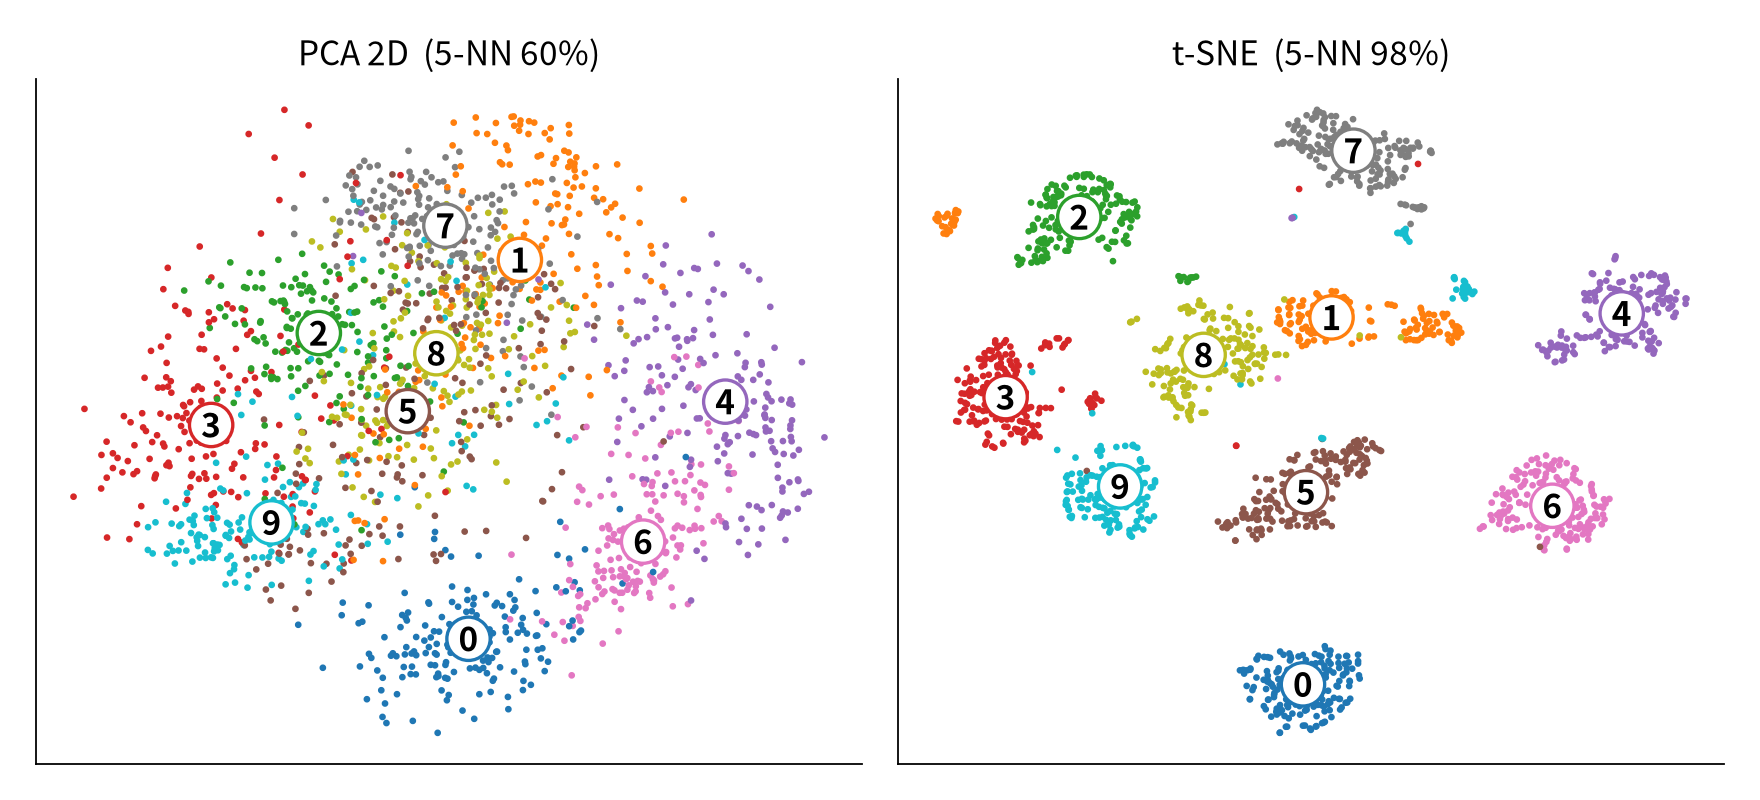
\includegraphics[width=0.74\linewidth]{ts_maps.png}\par\vskip0.1em
{\large 지도에서 가까운 5개로 숫자 맞히기 (5-NN): \quad PCA \kq{60\%} \quad t-SNE \kb{98\%}}\\[0.2em]
{\small 두 지도 모두 숫자 이름표는 쓰지 않았다 (색은 나중에 칠함)}
\vfill
\note{왼쪽이 PCA 두 축으로 그린 지도입니다. 0, 4, 6은 따로 보이지만 나머지 숫자는 서로 뒤엉켜 있습니다. 오른쪽이 오늘 배울 t-SNE로 그린 지도입니다. 0부터 9까지 섬처럼 갈라집니다. 얼마나 잘 갈라졌는지 재려고 지도에서 가장 가까운 5개 점의 숫자로 투표해 맞혀 보면, PCA 지도는 60퍼센트, t-SNE 지도는 98퍼센트입니다. 두 지도 모두 숫자 이름표는 쓰지 않았고, 색은 다 그린 뒤에 칠했습니다.}
\end{frame}

% --- 아이디어
\begin{frame}{아이디어: 이웃 관계를 지킨다}
\vfill
\centering
\renewcommand{\arraystretch}{1.6}
{\large\begin{tabular}{lll}
 & PCA & t-SNE (2008)\\\hline
지키려는 것 & 큰 퍼짐 (먼 거리) & \kb{가까운 이웃}\\
방법 & 직선 방향의 그림자 & 점을 하나씩 옮겨 가며 맞춘다 (경사 하강)\\
결과 & 축에 뜻이 있다 (PC1 = $\cdots$) & 축에 뜻이 없다, 무리가 보인다\\
새 점 & 바로 투영 & 다시 계산해야
\end{tabular}}\vskip0.8em
{\large ``64차원에서 가까운 점은 지도에서도 가깝게, 먼 점은 신경 쓰지 말자''}
\vfill
\note{PCA는 퍼짐이 큰 방향, 그러니까 먼 거리를 지키려 합니다. t-SNE는 2008년 반 데르 마턴과 힌튼이 발표했고, 가까운 이웃을 지키려 합니다. 64차원에서 가까운 점은 지도에서도 가깝게 두고, 먼 점들 사이의 거리는 크게 신경 쓰지 않습니다. 방법도 다릅니다. PCA는 직선 방향의 그림자를 내면 끝이지만, t-SNE는 지도 위 점들을 조금씩 옮겨 가며 이웃 관계를 맞춥니다. 경사 하강법이죠. 그래서 축에는 뜻이 없고, 새 점이 오면 다시 계산해야 합니다.}
\end{frame}

% --- 식
\begin{frame}{식으로: 두 가지 ``가까움'' 을 맞춘다}
\markpage{formula}
\vfill
\centering
\renewcommand{\arraystretch}{1.8}
{\large\begin{tabular}{ll}
64차원 (정규분포) & $p_{j|i} = \dfrac{\exp(-\|\mathbf{x}_i - \mathbf{x}_j\|^2 / 2\sigma_i^2)}{\sum_{k \ne i} \exp(-\|\mathbf{x}_i - \mathbf{x}_k\|^2 / 2\sigma_i^2)}, \quad p_{ij} = \dfrac{p_{j|i} + p_{i|j}}{2N}$\\
지도 (t 분포) & $q_{ij} = \dfrac{(1 + \|\mathbf{y}_i - \mathbf{y}_j\|^2)^{-1}}{\sum_{k \ne l} (1 + \|\mathbf{y}_k - \mathbf{y}_l\|^2)^{-1}}$\\
맞추기 & $\text{KL}(P \,\|\, Q) = \sum_{i \ne j} p_{ij} \log \dfrac{p_{ij}}{q_{ij}}$ \quad 를 지도 좌표 $\mathbf{y}$ 로 경사 하강
\end{tabular}}\\[0.4em]
{\small $\sigma_i$: 점마다 이웃이 약 \textbf{perplexity} 개 들어오도록 정한다 (빽빽한 곳은 좁게, 성긴 곳은 넓게)}
\vfill
\note{식으로 보면, 64차원에서 점 i가 점 j를 이웃으로 고를 확률 p를 정규분포 모양으로 정합니다. 가까울수록 크고, 합이 1이 되게 나눕니다. 양쪽 방향을 평균 내 p_ij를 만듭니다. 지도에서는 같은 일을 t 분포, 1 나누기 1 더하기 거리 제곱으로 합니다. 이게 q입니다. 그리고 두 분포의 차이, 14주차에 자세히 배울 KL 발산을 지도 좌표로 경사 하강해서 줄입니다. 시그마는 점마다 다르게, 이웃이 대략 perplexity 개 들어오도록 정합니다. 빽빽한 곳은 좁게, 성긴 곳은 넓게 보는 거죠.}
\end{frame}

% --- 손 계산 + 왜 t
\begin{frame}{손으로 한 번 · 왜 t 분포인가}
\markpage{hand}
\vfill
\begin{columns}[c]
\column{0.5\linewidth}\centering
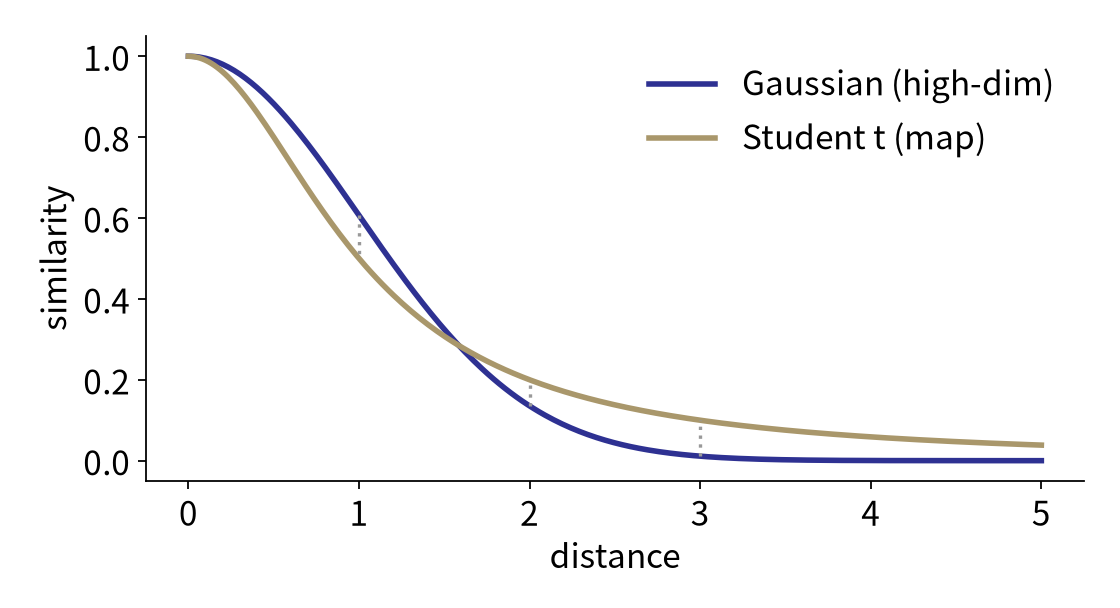
\includegraphics[width=\linewidth]{ts_kernel.png}
\column{0.48\linewidth}
{\large 이웃 셋까지 거리 1, 2, 3}\\[0.3em]
\renewcommand{\arraystretch}{1.3}
{\normalsize\begin{tabular}{lccc}
 & 1 & 2 & 3\\\hline
$e^{-d^2/2}$ & 0.607 & 0.135 & 0.011\\
나눠 합 1 & \kb{0.81} & 0.18 & \kq{0.01}\\\hline
$1/(1 + d^2)$ & 0.5 & 0.2 & 0.1\\
나눠 합 1 & 0.625 & 0.25 & \kb{0.125}
\end{tabular}}\\[0.5em]
{\small t 분포는 꼬리가 두껍다: 조금 먼 점도 몫이 남는다}
\end{columns}\vskip0.3em
\centering{\large 작은 몫을 맞추려면 지도에서는 먼 점을 \kb{더 멀리} $\to$ 섬 사이에 틈}\\[0.1em]
{\small 64차원의 이웃을 2차원에 다 넣을 자리가 없는 문제 (crowding problem)}
\vfill
\note{점 하나에서 이웃 셋까지 거리가 1, 2, 3이라고 합시다. 정규분포 모양으로 재면 0.607, 0.135, 0.011이고, 합이 1이 되게 나누면 0.81, 0.18, 0.01입니다. 거리 3인 점은 거의 몫이 없습니다. t 분포로 재면 0.5, 0.2, 0.1, 나누면 0.625, 0.25, 0.125입니다. t 분포는 꼬리가 두꺼워서 조금 먼 점도 몫이 남습니다. 그러면 64차원의 작은 p를 지도에서 맞추려면 그 점을 지도에서는 더 멀리 둬야 합니다. 그래서 무리 사이에 틈이 생깁니다. 64차원의 넓은 이웃들을 2차원에 다 넣을 자리가 없는 문제, crowding problem을 이렇게 풉니다. 원래 SNE는 지도에도 정규분포를 썼고, t로 바꾼 게 t-SNE의 t입니다.}
\end{frame}

\section{설정 · 주의}
% --- perplexity
\begin{frame}{설정에 따라 달라진다: perplexity}
\vfill
\centering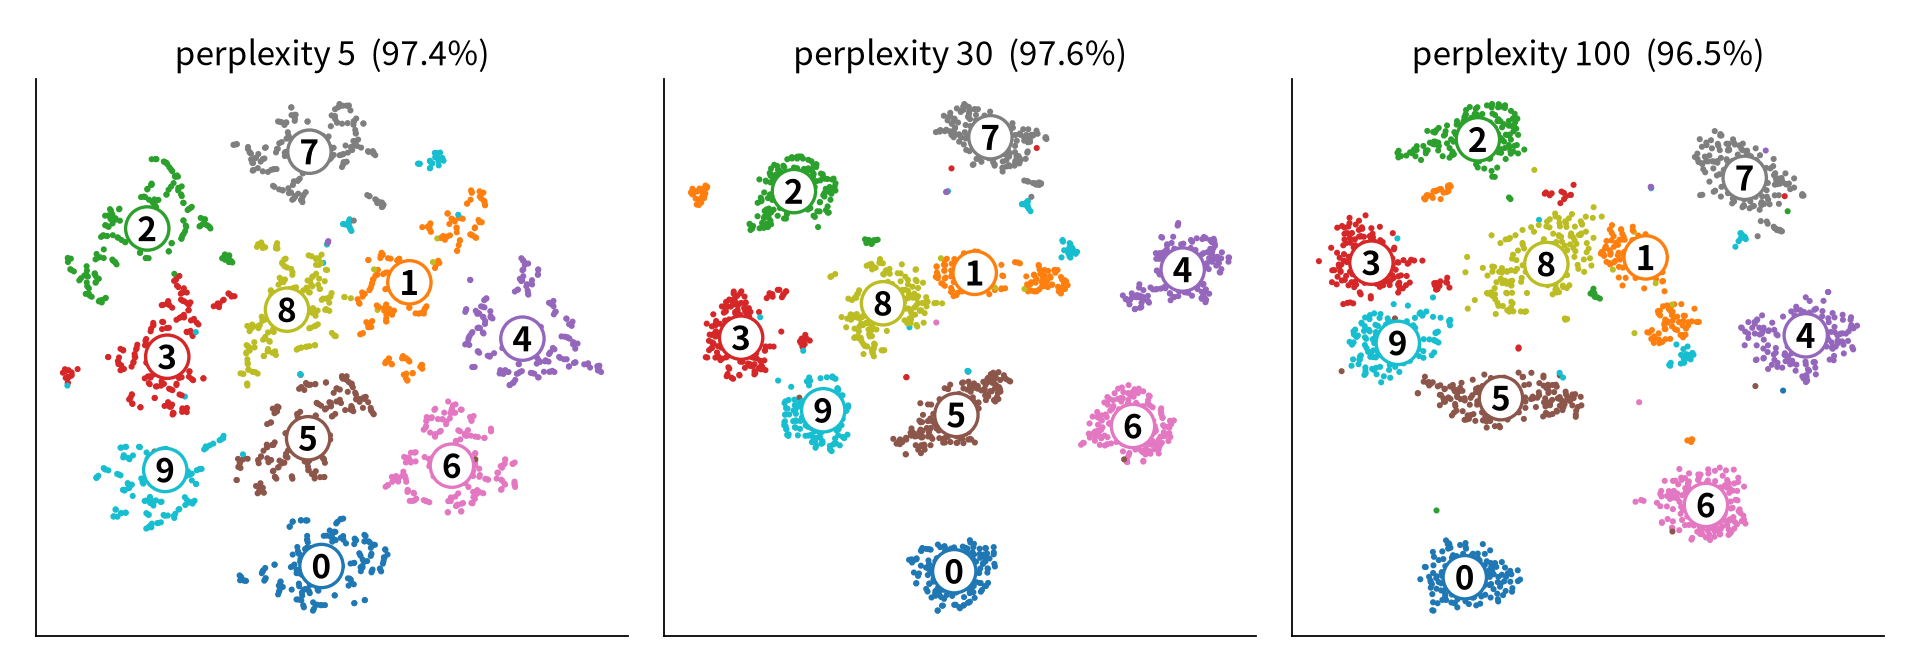
\includegraphics[width=0.92\linewidth]{ts_perp.png}\par\vskip0.2em
{\large perplexity = 점마다 대략 몇 개를 이웃으로 볼지 \quad (보통 5 $\sim$ 50)}\\[0.2em]
{\large 작으면 잘게 쪼개지고, 크면 전체 모양을 더 본다 \quad (5-NN 은 97\% 안팎)}
\vfill
\note{t-SNE의 가장 중요한 설정이 perplexity입니다. 점마다 대략 몇 개를 이웃으로 볼지를 정하고, 보통 5에서 50 사이를 씁니다. 5로 하면 작은 무리로 잘게 쪼개지고, 100으로 하면 전체 모양을 더 봅니다. 지도에서 가까운 5개로 맞히는 정확도는 셋 다 97퍼센트 안팎이지만, 지도의 모양은 꽤 다릅니다. 그래서 t-SNE 지도는 설정을 몇 가지 바꿔 보고 해석해야 합니다.}
\end{frame}

% --- 주의: 크기
\begin{frame}{주의 1: 섬의 크기는 뜻이 없다}
\markpage{caveat}
\vfill
\centering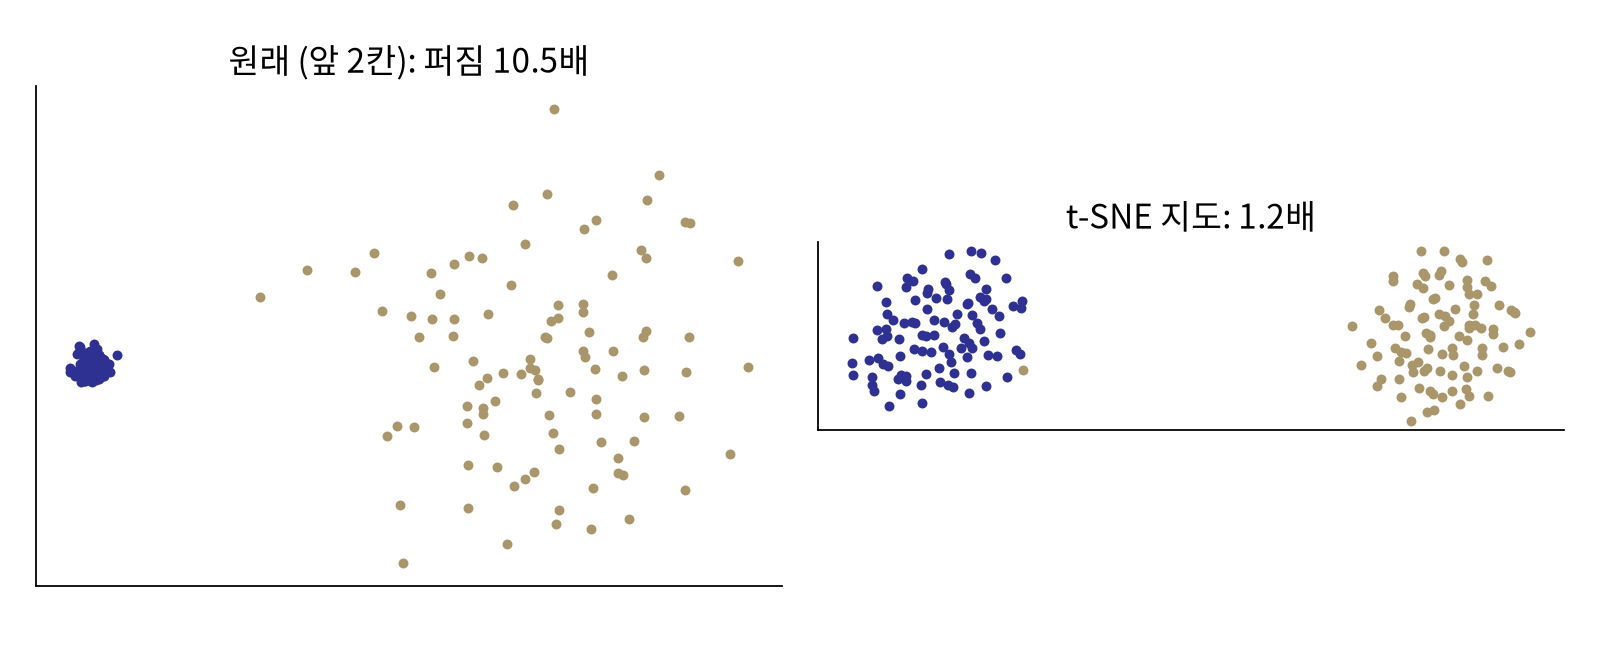
\includegraphics[width=0.78\linewidth]{ts_two.png}\par\vskip0.1em
{\large 10차원 두 무리, 퍼짐 \kq{10.5배} 차이 $\to$ 지도에서는 \kb{1.2배}}\\[0.2em]
{\large 점마다 $\sigma_i$ 를 따로 정하니 빽빽한 무리는 늘고 성긴 무리는 준다}
\vfill
\note{t-SNE 지도를 볼 때 주의할 점이 있습니다. 첫째, 섬의 크기는 뜻이 없습니다. 10차원에 두 무리를 만들었는데, 노란 무리가 파란 무리보다 10.5배 넓게 퍼져 있습니다. 그런데 t-SNE 지도에서는 1.2배, 거의 같은 크기입니다. 점마다 이웃이 perplexity 개 들어오도록 시그마를 따로 정하니까, 빽빽한 무리는 늘어나고 성긴 무리는 줄어들어 비슷한 크기가 됩니다.}
\end{frame}

% --- 주의: 거리, 시드
\begin{frame}{주의 2: 섬 사이 거리 · 실행마다 다른 지도}
\vfill
\centering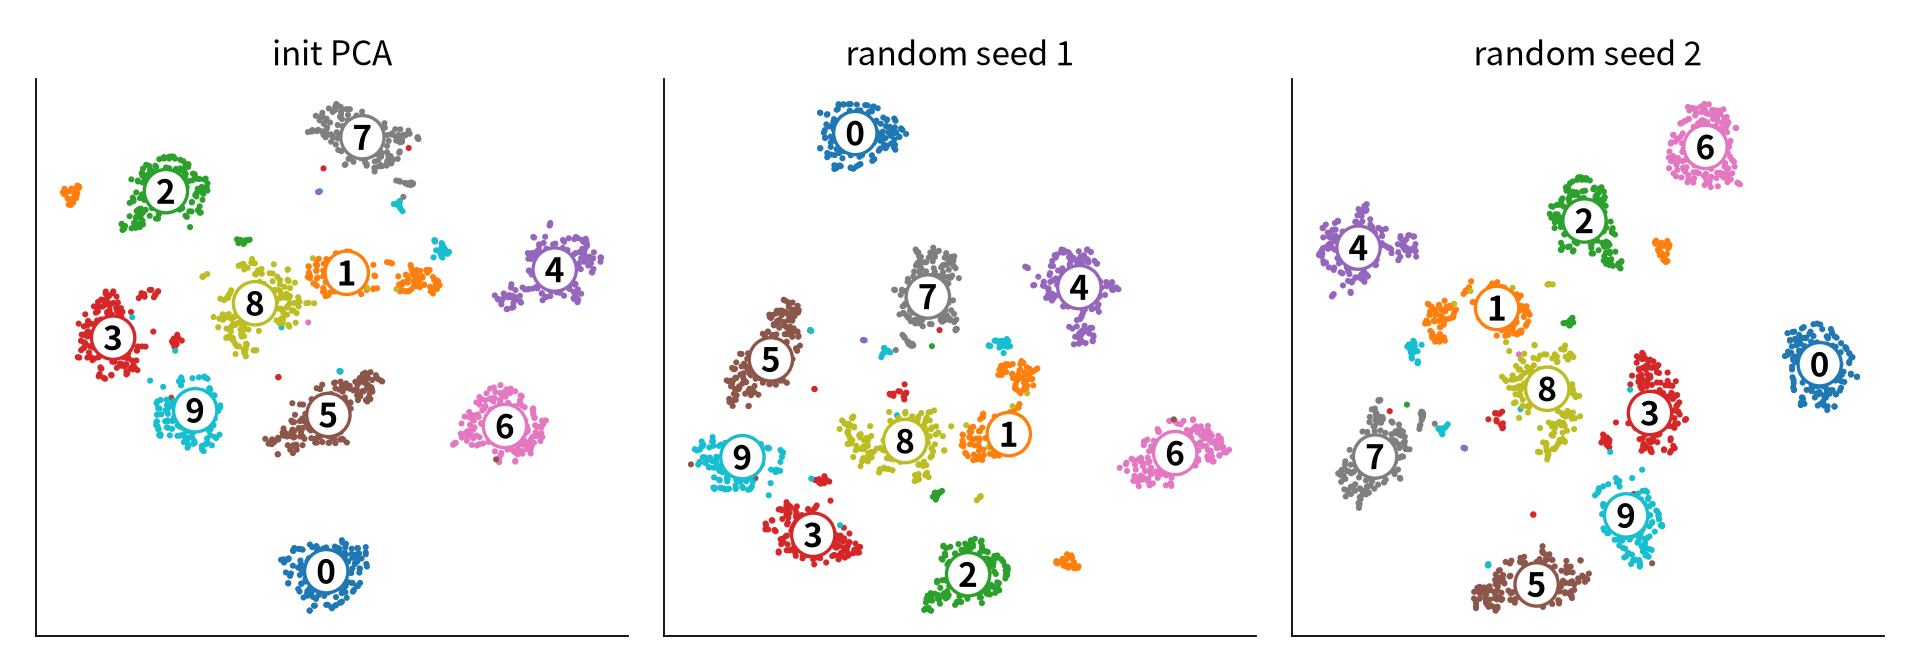
\includegraphics[width=0.86\linewidth]{ts_seeds.png}\par\vskip0.2em
{\large 시작점만 바꿨다 \quad 섬은 그대로, \textbf{배치}는 제각각 (5-NN 97 $\sim$ 98\%)}\\[0.2em]
{\large 섬 사이 거리 · 위치로 ``0 과 6 이 가깝다'' 고 결론 내리지 말 것}\\[0.1em]
{\small Wattenberg, Viégas, Johnson (2016) ``How to Use t-SNE Effectively'' (Distill)}
\vfill
\note{둘째, 섬 사이의 거리와 위치도 뜻이 거의 없습니다. 같은 데이터, 같은 설정으로 시작점만 바꿔 세 번 그렸습니다. 섬들은 그대로 갈라지지만, 어디에 놓이는지는 매번 다릅니다. 그러니 이 지도에서 0과 6이 가깝다 같은 결론을 내리면 안 됩니다. 무리가 있다는 것, 어떤 점이 어느 무리에 속하는지까지만 믿으세요. Distill의 How to Use t-SNE Effectively라는 글에 이런 예가 잘 정리돼 있습니다.}
\end{frame}

% --- 쓰임
\begin{frame}{어디에 쓰나}
\vfill
\centering
\renewcommand{\arraystretch}{1.5}
{\large\begin{tabular}{ll}
신경망 들여다보기 & 중간층 벡터 (임베딩) 를 지도로: 비슷한 것끼리 모였나?\\
단일 세포 유전체 & 세포 수만 개 × 유전자 2만 개 $\to$ 세포 종류가 섬으로\\
단어 · 문서 & word2vec · BERT 벡터를 지도로 (다음 덱들)\\
UMAP (2018) & 비슷한 생각, 더 빠르고 전체 모양을 조금 더 지킨다
\end{tabular}}\vskip0.8em
{\large 지도는 \textbf{보기 위한} 것: 지도 좌표로 분류 · 군집을 하지는 않는다}
\vfill
\note{t-SNE는 주로 들여다보는 데 씁니다. 신경망의 중간층 벡터를 지도로 그려 비슷한 것끼리 모였는지 확인하고, 단일 세포 유전체 분석에서는 세포 수만 개를 유전자 2만 개로 잰 데이터를 지도로 그려 세포 종류를 섬으로 봅니다. 다음 덱들에서 다룰 word2vec이나 BERT의 단어 벡터도 이렇게 그립니다. 2018년의 UMAP은 비슷한 생각인데 더 빠르고 전체 모양을 조금 더 지킵니다. 다만 지도는 보기 위한 것입니다. 지도 좌표로 분류나 군집을 하면 앞에서 본 왜곡을 그대로 믿게 됩니다.}
\end{frame}

\section{연습}
% --- 문제풀이
\begin{frame}{문제풀이}
\vfill
\begin{enumerate}
\item 이웃 거리가 0 과 1 일 때 t 분포 유사도 $1/(1 + d^2)$ 는? 합이 1 이 되게 나누면?\vskip0.8em
\item 정규분포로는 거리 3 인 점의 몫이 0.01, t 분포로는 0.125 였다. 지도에서 0.01 을 맞추려면 그 점을 가깝게 둬야 할까, 멀게 둬야 할까?\vskip0.8em
\item t-SNE 지도에서 섬 A 가 섬 B 보다 3배 크다. ``A 가 3배 다양하다'' 고 말할 수 있나?\vskip0.8em
\item PCA 와 달리 t-SNE 는 새 데이터 한 장을 바로 지도에 올릴 수 없다. 왜일까?
\end{enumerate}
\vfill
\note{1번 답. 1과 0.5이고, 나누면 3분의 2와 3분의 1입니다. 2번 답. 멀게 둬야 합니다. t 분포는 꼬리가 두꺼워 웬만한 거리에서도 몫이 크니, 0.01까지 줄이려면 훨씬 멀리 보내야 합니다. 그래서 무리 사이에 틈이 생깁니다. 3번 답. 말할 수 없습니다. 점마다 시그마를 따로 정해 크기를 비슷하게 만들기 때문에, 섬 크기는 원래 퍼짐을 반영하지 않습니다. 4번 답. t-SNE는 점들의 좌표 자체를 경사 하강으로 맞춘 것이지, 64차원에서 2차원으로 가는 함수를 배운 게 아니기 때문입니다.}
\end{frame}

% --- 실습
\begin{frame}{실습}
\vfill
\centering\begin{tabular}{rl}
\large 1 & 정규분포 vs t 분포 유사도 손 계산, KL 발산 재기\\[0.5em]
\large 2 & 손글씨 숫자 PCA 지도 vs \texttt{sklearn TSNE} 지도 $\to$ 5-NN 60\% vs 98\%\\[0.5em]
\large 3 & perplexity · 시드 바꾸기, 크기가 다른 두 무리 실험
\end{tabular}\vskip1em
\href{https://colab.research.google.com/github/SuminHan/book-ml/blob/main/slides/v2/ml1/week14/tsne/lab/tsne.ipynb}{\textcolor{ksagolddk}{▶ Colab에서 실습 노트북 열기}}
\vfill
\note{실습은 세 부분입니다. 첫째, 정규분포와 t 분포 유사도를 손 계산하고 KL 발산을 재 봅니다. 둘째, 손글씨 숫자를 PCA와 sklearn TSNE로 지도에 그리고, 가까운 5개로 맞히는 정확도를 비교합니다. 셋째, perplexity와 시드를 바꿔 보고, 크기가 다른 두 무리 실험을 합니다.}
\end{frame}

\section{정리}
% --- 정리
\begin{frame}{정리}
\vfill
\centering\large\begin{tabular}{l}
\textbf{t-SNE}: 64차원에서 \kb{가까운 이웃}은 지도에서도 이웃으로 (2008)\\[0.5em]
고차원은 정규분포, 지도는 꼬리가 두꺼운 \textbf{t 분포} $\to$ KL 발산을 경사 하강\\[0.5em]
숫자 1,797장: PCA 지도 60\% $\to$ t-SNE 지도 98\% (가까운 5개로 맞히기)\\[0.5em]
주의: 섬 크기 (10.5배 $\to$ 1.2배) · 섬 사이 거리 · 배치에는 뜻이 없다
\end{tabular}
\vfill
\note{정리합니다. t-SNE는 고차원에서 가까운 이웃을 지도에서도 이웃으로 두는 지도 그리기 방법입니다. 고차원에서는 정규분포로, 지도에서는 꼬리가 두꺼운 t 분포로 가까움을 재고, 두 분포의 KL 발산을 경사 하강으로 줄입니다. 손글씨 숫자 지도에서 가까운 5개로 맞히기는 PCA 60퍼센트, t-SNE 98퍼센트였습니다. 다만 섬의 크기, 섬 사이 거리, 배치에는 뜻이 없습니다. 10.5배 차이 나는 무리도 지도에서는 1.2배였습니다.}
\end{frame}
\end{document}
